% Define name of author (me).
\newcommand{\theauthor}{Vincent C. Mader}

% Define path to figures.
\newcommand{\pathToFigures}{../../../v4_final/msc-thesis.py/out/figures/}
\graphicspath{ {\pathToFigures} {./figures} }

% Remove indentation for new paragraphs.
\setlength\parindent{0pt}

% Define command for highlighting TODOs in document.
\newcommand{\todo}[1]{\textcolor{red}{TODO(}#1\textcolor{red}{)}}
\newcommand{\assume}[1]{\textcolor{blue}{ASSUME:} #1}

% Define commands for partial & total differentials & derivatives.
\newcommand{\dd}[0]{ \text{d} }
\newcommand{\del}[0]{ \partial }
\newcommand{\pderiv}[2]{ \frac{\del #1}{\del #2} }
\newcommand{\deriv}[2]{ \frac{\dd #1}{\dd #2} }

% Define path to file containing references.
\addbibresource{postface/references/references.bib}

% Define page style `plain` used for "new-chapter" pages.
\fancypagestyle{plain}{%
}
% % Define page style `NoHeader` used for disabling page header.
\fancypagestyle{NoHeader}{%
    \fancyhf{}
    \renewcommand{\headrulewidth}{0pt}
}
% Define page style `Fancy` used for enabling page header.
\fancypagestyle{Fancy}{
    \fancyhf{}                % Clear default settings
    \fancyhead[L]{\leftmark}  % Chapter title on the left
    \fancyhead[R]{\thepage}   % Page number on the right
    \renewcommand{\headrulewidth}{0.5pt}
}
% Re-define (decrease) font-size for chapter number & title.
\chapternumberfont{\LARGE} 
\chaptertitlefont{\huge}

\crefformat{figure}{#2figure~#1#3}
\crefformat{section}{#2section~#1#3}
\crefformat{subsection}{#2section~#1#3}
\crefformat{chapter}{#2chapter~#1#3}
\crefformat{equation}{#2equation~(#1)#3}

% \newcommand{\citepretty}[1]{\hyperref[{#1}]{\cite{#1}}}









\newcommand{\colorbar}[2]{
    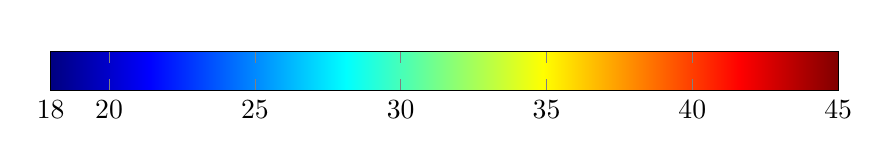
\begin{tikzpicture}
        \begin{axis}[
            hide axis,
            scale only axis,
            height=0pt,
            width=0pt,
            colormap/jet,
            colorbar horizontal,
            point meta min=18,
            point meta max=45,
            colorbar style={
                width=10cm,
                xtick={18,20,25,...,45}
            }]
            \addplot [draw=none] coordinates {(0,0)};
        \end{axis}
    \end{tikzpicture}
}
